\documentclass[]{article}
\usepackage[pdftex]{graphicx}  
\usepackage{color}
\usepackage{hyperref}

\begin{document}

%---------------------------------------------------------%
%FRONT PAGE
%---------------------------------------------------------%
\section*{BIS101 Fall 2013. Exam \#1}
You are welcome to use standard academic resources available to you (books, articles, the internet), but do not consult with other students.  Please keep your answers brief, but you must show your work for full credit.  The test is 100 points. The exam is due Thursday Oct 31 at 5pm.  It can only be turned in electronically via SmartSite.  SmartSite will not accept exams after 5pm, and late exams cannot be turned in by other means. {\bf Do not wait until the last minute to turn your exam in; problems with SmartSite, internet connections, or your computer are not acceptable reasons for missing the deadline.}  Your exam will not be graded unless this front page is turned in with your name, student ID, and your signature below.  This page may be turned in in person or along with your exam. By signing, you are verifying that you understand the exam deadline and agree to abide by the UCD Code of Academic Conduct \url{http://sja.ucdavis.edu/cac.html}.  \\
\vspace{2cm} \\

\begin{tabular}{lll}
& Name & \underline{\hspace{5cm}} \\
\vspace{2cm} \\
& Student ID & \underline{\hspace{5cm}} \\
\vspace{2cm} \\
& Signature & \underline{\hspace{5cm}} \\
\vspace{2cm} \\
\end{tabular}

%---------------------------------------------------------%
%BEGIN PROBLEMS
%---------------------------------------------------------%
\begin{enumerate}

%---------------------------------------------------------%
%PEDIGREE/MENDEL
%---------------------------------------------------------%
\newpage
%10min
%dad #3 is WT
%mom is WT because likelihood of having 6 sons w/o dissease is <<20%
%0 0 0.5 0.5
\item Figure \ref{dogigree} is a pedigree of miniature schnauzers (a dog breed). Female \#2 has already had one litter, and male \#3 has already sired two offspring with female \#4. A breeder is interested in mating female \#2 and male \#3, but is worried about a recessive X-linked disorder called Von-Willibrands disease in their offspring. Answer the following:

\begin{enumerate}
\item What are the genotypes of dogs \#1, \#3, and \#4? (4pts)
\item The breeder had female \#2 tested for the disease, and the test result suggested she was a carrier. The test is imperfect, however, and ~20\% of the time returns an incorrect positive result. You are a geneticist brought in to advise the breeder. What is the most likely genotype of dog \#2? Explain how you reach this conclusion. (4pts)
\item Given the most likely genotypes for dogs \#2 and \#3, what is the probability that dogs \#2 and \#3 will have: (2 pts)
\begin{enumerate}
\item A male puppy with Von-Willibrands disease?
\item A female puppy with Von-Willibrands disease?
\item A normal female puppy?
\item A normal male puppy?
\end{enumerate}
\end{enumerate}

\begin{figure*}[h]
  \begin{center}
   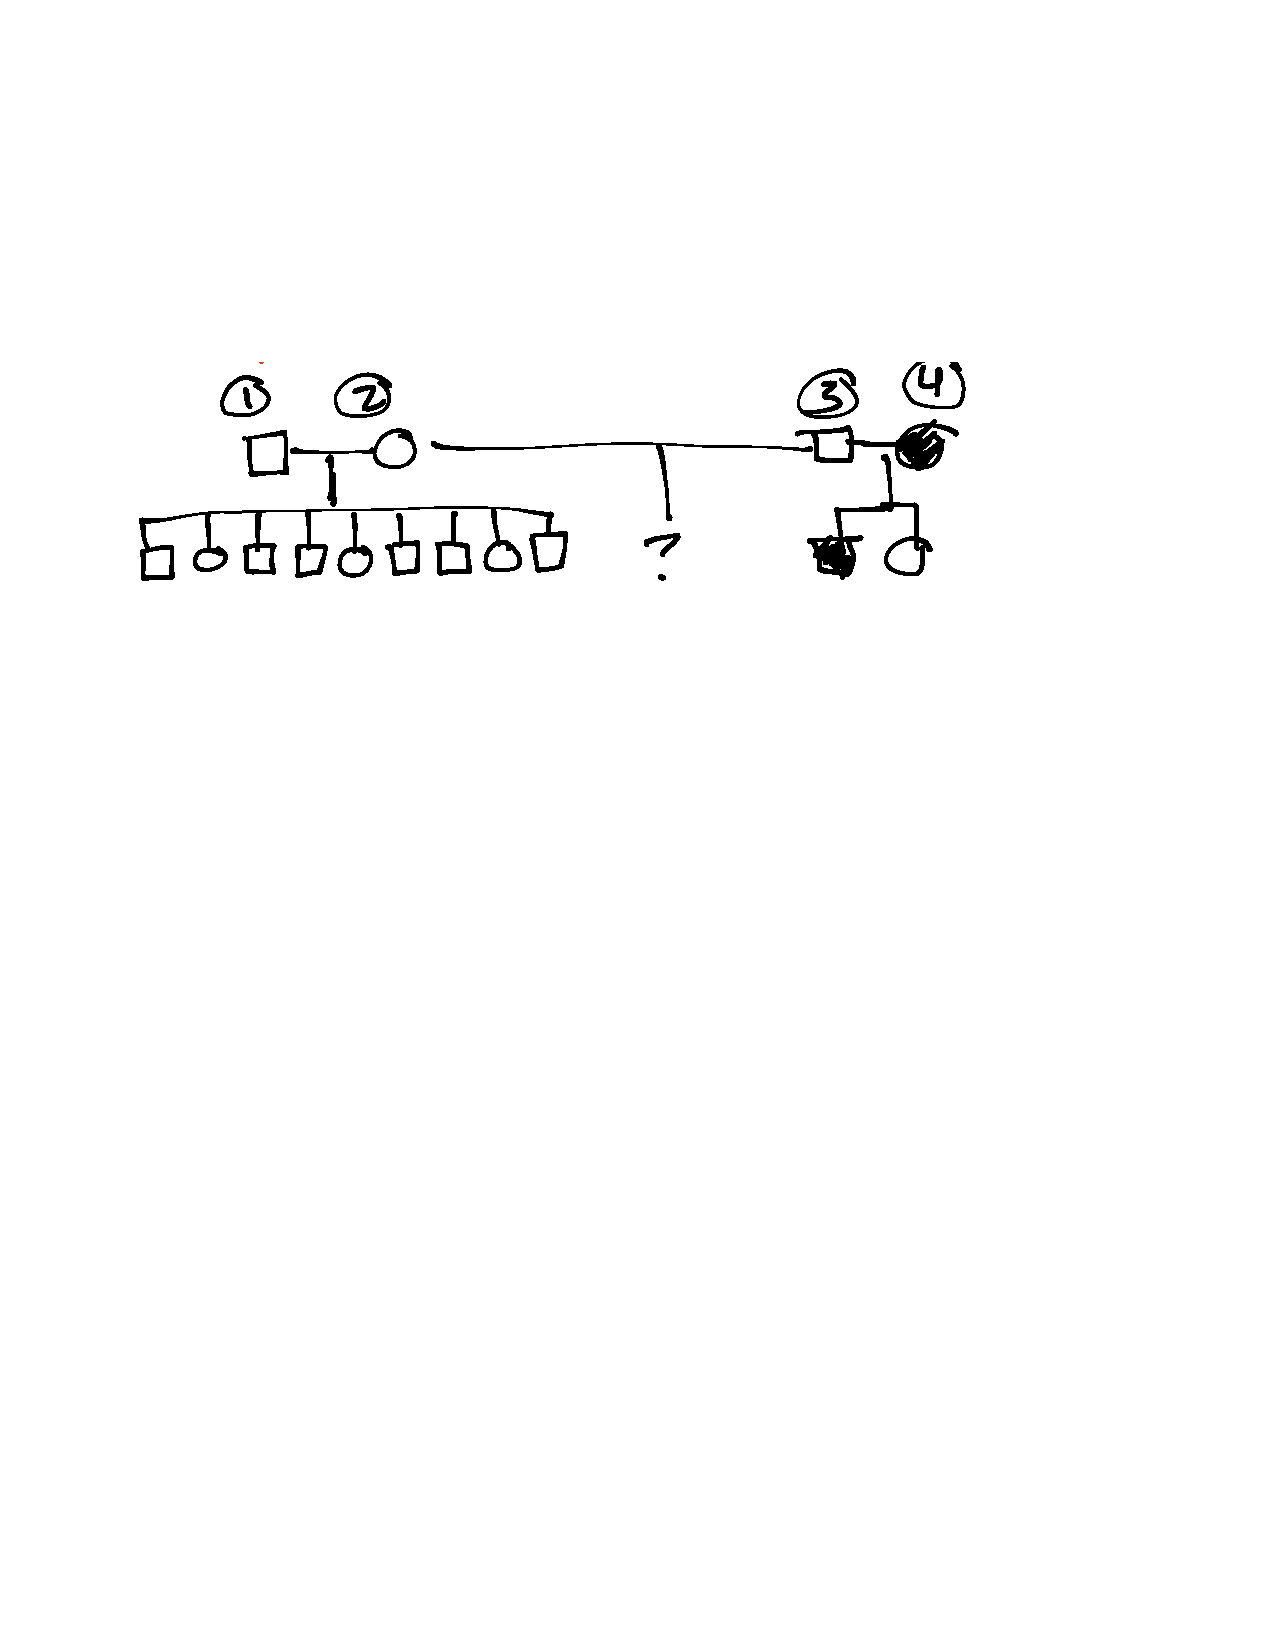
\includegraphics[width=130mm]{images/pedigree_test.pdf}
\caption{A pedigree of miniature schnauzers. Filled symbols (square=male, circle=female) represent dogs with Von-Willibrands disease. Empty symbols are dogs with wild-type phenotypes.}
\label{dogigree}
  \end{center}
\end{figure*}

%---------------------------------------------------------%
%QUANTITATIVE GENETICS
%---------------------------------------------------------%
\newpage
%8 mins
% variance is either 7.089506 or 7.506536
%$H^2=(Vp-Ve)/Vp so (7.09-3.2)/7.09 or (7.5-3.2)/7.5 (anything between 54 and 58% credit)
\item You are interested in understanding the genetics of furriness in rabbits. You recruit 18 rabbit owners to bring in their bunnies for measurement.  Each bunny's fluffiness is measured on a scale of 1 (no hair) to 10 (see \url{http://goo.gl/5fssLD} for an example of 10). Phenotypes for all 18 bunnies are shown in Table \ref{fluffy}. 

\begin{enumerate}
\item Calculate the phenotypic variance for fluffiness (5 pts).
\item In a separate study, you measure the fluffiness of a set of rabbit quadruplets that were sold by a breeder to 4 different families.  The phenotypic variance among these four genetically identical rabbits is 3.2. If these families are representative of the environments of the rabbits in Table \ref{fluffy}, use these data and the phenotypic variance in part (a) to calculate the broad sense heritability of fluffiness (5 pts).

%Their phenotypes are shown in Table \ref{clones}. Using these data, calculate the broad sense heritability of fluffiness in rabbits (6 pts).
\end{enumerate}

\begin{table}[h]
\caption[]{Rabbit phenotypes.}
\begin{center}
\begin{tabular}{ll}
Rabbit Name & Fluffiness \\  \hline
Baby & 2\\
Baggins & 8\\
Bambi & 9\\
Barbie & 10\\
Basil & 7\\
Bella & 2\\
Benny & 7\\
Big Boy & 5\\
Big-Ears & 2\\
Binky & 10\\
Bluebell & 8\\
Boo Boo & 8\\
Buddy & 4\\
Bugs & 4\\
Bun Bun & 4\\
Bunnicula & 3\\
Bunzilla & 6\\
Buttercup & 4\\
\end{tabular}
\end{center}
\label{fluffy}
\end{table}

%\begin{table}[h!]
%\caption[]{Quadruplet rabbit phenotypes.}
%\begin{center}
%\begin{tabular}{ll}
%Rabbit Name & Fluffiness \\  \hline
%Oliver & 7\\
%Ollie & 8\\
%Oreo & 9\\
%Oscar & 9\\
%\end{tabular}
%\end{center}
%\label{clones}
%\end{table}

%---------------------------------------------------------%
%INTERACTION/EPISTASIS
%---------------------------------------------------------%
\newpage
%8 minutes
% both recessive homozygotes at different loci
\item Abscisic acid is an important regulator of seed maturation and germination in plants. You have two mutant maize plants that make insufficient levels of abscisic acid and thus their kernels germinate prematurely on the cob. When you self the first mutant it produces 345 mutant offspring. When you cross the second mutant to a wild-type plant all of the F1 are wild-type, and selfing the F1 results in 265 wild-type and 89 mutant offspring.  When you cross both original mutants together they produce 563 wild-type offspring.  Draw the genotypes of both mutant lines and the dominance of the alleles involved (10 pts).

%---------------------------------------------------------%
% SCHEMPSKE \& BRADSHAW (1999)
%---------------------------------------------------------%
\newpage
% 5 minutes
%High (say above 60%) because single gene of large effect. Should be <100% because there will be environmental variation.
\item The following questions refer to the paper by Schemske and Bradshaw (1999). Carotenoid content in \emph{Mimulus} flowers is controlled by a single Mendelian locus called \emph{yup}. At this locus the \emph{M. cardinalis} allele is recessive to the \emph{M. lewissii} allele. 
\begin{enumerate}
\item In a population of F2 plants generated from a cross between \emph{M. lewissii}  and \emph{M. cardinalis}, provide an estimate as to what you think the broad sense heritability for the orange/red color would be (\emph{hint: no calculations are needed to answer this question}) (3 pts).
\item Provide an explanation for your answer in part (a) (3 pts).
\end{enumerate}

%---------------------------------------------------------%
% LIU ET AL (2012)
%---------------------------------------------------------%
\newpage
% 15 minutes
\item Figure \ref{homologs} shows the karyotype of two individual plants of the genus\emph{Silene}.  The duplicated gene shown codes for an inorganic compound which causes plant tissue to appear significantly darker. The copy on chromosome 1 is expressed only in leaves, and the copy on chromosome 2 is expressed only in flower petals. Both loci are haplosufficient. (\emph{hint: reading Liu et al. 2012 may be helpful for figuring out this problem}).

\begin{enumerate}
\item Draw the karyotype and phenotype of the F1 and all possible F2 (6 pts). %9 genotypes
\item I make a mutant version of I207 in the lab which has pale flowers and breeds true. Sequencing shows this mutant is homozygous for a mutation in the gene on chromosome 2 shown in figure \ref{homologs}. If I cross this mutant line with the F1 between wild-type I207 and B97, what proportion of the offspring will have pale flowers (4 pts)? % 50%
\end{enumerate}

\begin{figure*}[h]
  \begin{center}
   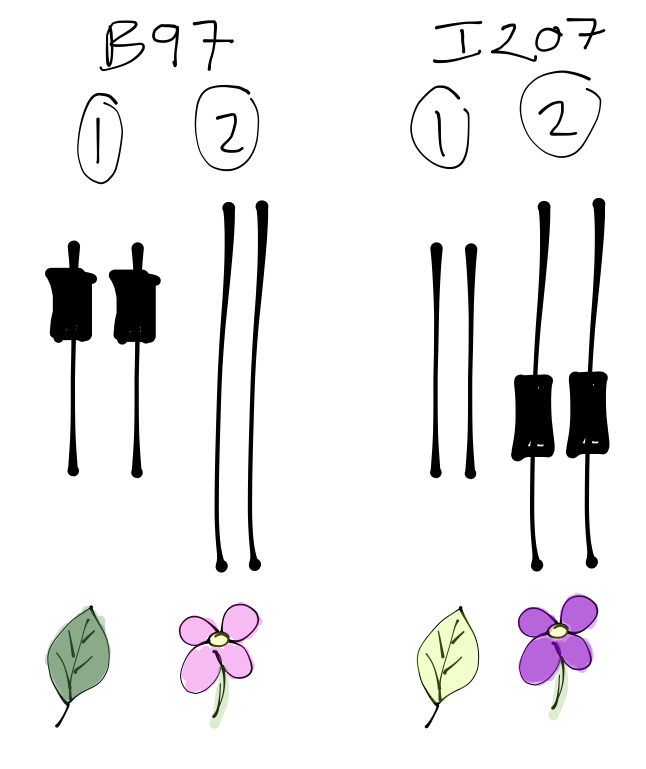
\includegraphics[width=80mm]{images/homologs.png}
    \caption{Karyotype for chromosomes 1 and 2 of \emph{Silene} lines B97 and I207. Boxes on each chromosome represent the presence of a gene of interest (the absence of a box signifies that the gene is not present on that chromosome). The flower and leaf phenotype of each line is shown below the karyotype: B97 has dark leaves and pale flowers and I207 has pale leaves and dark flowers.} 
\label{homologs}
  \end{center}
\end{figure*}

%---------------------------------------------------------%
% GENOMICS/PHYLOGENETICS
%---------------------------------------------------------%
% 12 minutes

\newpage
\item Use the phylogeny of the gene \emph{ahbp3} shown in figure \ref{duplicates} to answer the following questions.

\begin{enumerate}
\item What term would you use to describe the relationship between the  rice \#5 and \emph{Sorghum} \#1 copies of \emph{ahbp3} in figure \ref{duplicates}  (2 pts)? 
%paralogs
\item What evolutionary process would you ascribe to gene copies \#3 and \#7 in \emph{Zea} in figure \ref{duplicates} (2 pts)?
%subfunctionalization
\item Is \emph{Zea} copy \#2 or copy \#3 more in figure \ref{duplicates} more likely to be in a syntenic position relative to \emph{Sorghum} \#1 (2 pts)?
%pink/blue
\item In what tissue(s) do you think the gene copy ancestral to all the plants shown was expressed (2 pts)?
%roots and leaves
\item If you compare the sequence of the \emph{Zea} copy \#2 of \emph{ahbp3} expressed only in flowers to the \emph{ahbp3} locus in \emph{Agave} (\#9), what do you predict will be the relationship between nonsynonymous substitutions and synonymous substitutions (2 pts)?
%dn/ds >1
\end{enumerate}

\begin{figure*}[h]
  \begin{center}
   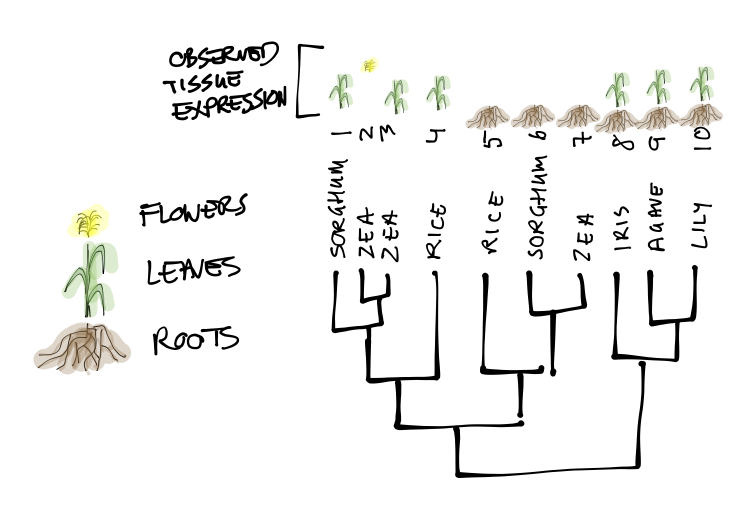
\includegraphics[width=110mm]{images/examfig2.png}
    \caption{Shown is a phylogenetic tree of the sequences of the \emph{ahbp3} locus in a groups of plants. The genus \emph{Zea} has 3 copies of this gene, while\emph{Sorghum} and rice each have two. Above the phylogeny is shown the tissues in which each copy is expressed. Genes are numbered for reference in the questions above.} 
\label{duplicates}
  \end{center}
\end{figure*}

%---------------------------------------------------------%
% 8 ET AL (2013)
%---------------------------------------------------------%
\newpage
%10mins
%Ne*s > 1
\item Johnston et al. (2013) investigate the genetic variation of horn size in Soay sheep. Explain how they were able to rule out genetic drift as an explanation for the observed variation at the Ho locus (6 pts).

%---------------------------------------------------------%
% LINKAGE MAPPING
%---------------------------------------------------------%
\newpage
%25 mins
% 38 distance so 15.5% for parental types and 9.5% for recombinants
\item You cross two inbred lines of tomato: a hairy, jointed, tall plant with a hairless, dwarf, and jointless plant.  The F1 are all hairy, jointed, and tall.  Write out the genotype and phenotype ratios in the progeny of a cross between this F1 and a hairless, dwarf, and jointless tester.  Use Figure \ref{map} (also Figure 4-13c in your book) to help answer the question (10 pts).

\begin{figure*}[h]
  \begin{center}
   \includegraphics[width=110mm]{griffiths/ch04/figure_04_13c.jpg}
    \caption{A genetic map of tomato. } 
\label{map}
  \end{center}
\end{figure*}


%---------------------------------------------------------%
% CHROMOSOMAL EVOLUTION
%---------------------------------------------------------%
\newpage
% 10 mins
\item Use Figure \ref{map} (also Figure 4-13c in your book) to answer the following question. An inversion occurs on chromosome 7.  The first inversion breakpoint is 7cM from the green-base/uniform locus and the second breakpoint is 5cM from the xanthophyllous locus. The inversion includes both the hairy locus and the tangerine locus. Draw the inverted chromosome with genetic distances. (6 pts).


%---------------------------------------------------------%
% POPULATION GENETICS
%---------------------------------------------------------%
\newpage
%5 mins
\item You genotype a sample of pollen grains from a population of wild tomatoes at the \emph{jointless} and the \emph{leafy} loci. The observed haploid genotypes are shown in Table \ref{tomaters}. 

\begin{enumerate}
\item What are the allele frequencies of the j and lf aleles? (2 pts) 
\item Are these loci in linkage {\bf disequilibrium}? (2 pts)
\item Predict the genotype frequencies of diploid tomato plants in the next generation at each locus (2 pts).
\item If the \emph{J} is deleterious and completely dominant, write out the relative fitnesses of the three genotypes at the \emph{jointless} locus (2 pts).
\item If \emph{j lf} gametes begin to have low fertilization success
\begin{enumerate}
\item What will happen to the frequency of each allele over many generations (2 pts)?
\item What will happen to linkage disequilibrium between the loci (2 pts)?
\end{enumerate} 
\end{enumerate}

\begin{table}[h]
\caption[]{Tomato haploid genotypes.}
\begin{center}
\begin{tabular}{ll}
Genotype & Number \\  \hline
J Lf & 63\\  
J lf & 7\\
j Lf & 27\\
j lf & 3\\

\end{tabular}
\end{center}
\label{tomaters}
\end{table}

%---------------------------------------------------------%
% IBARRA-LACLETTE ET AL (2013)
%---------------------------------------------------------%
\newpage
%5 mins
\item Ibarra-Laclette studied the genome of a carnivorous plant, \emph{Utricularia gibba}.  They found a small genome, with an average total number of genes.  They use comparative genomics to answer questions about the genomic history of \emph{U. gibba}.  Use the haploid ancestral block of genes in shown in Figure \ref{minute} to answer these questions.

\begin{enumerate}
\item If the ancestral gene block undergoes 2 whole genome duplications, circle the correct response for each (4 pts):\\

Total copy number of gene A:\hspace{5mm}1\hspace{5mm}2\hspace{5mm}3\hspace{5mm}4\\
Total copy number of gene B:\hspace{5mm}1\hspace{5mm}2\hspace{5mm}3\hspace{5mm}4\\
Is synteny retained?\hspace{5mm}yes\hspace{5mm}no\\
Total amount of DNA:\hspace{5mm}up\hspace{5mm}down\hspace{5mm}same\\

\item If gene B is cut out and moved to a new chromosome via the action of transposable elements, circle the correct response for each (4 pts):\\

Total copy number of gene A:\hspace{5mm}1\hspace{5mm}2\hspace{5mm}3\hspace{5mm}4\\
Total copy number of gene B:\hspace{5mm}1\hspace{5mm}2\hspace{5mm}3\hspace{5mm}4\\
Is synteny retained?\hspace{5mm}yes\hspace{5mm}no\\
Total amount of DNA:\hspace{5mm}up\hspace{5mm}down\hspace{5mm}same\\
\item Draw the resulting gene block after the ancestral gene block experiences fractionation without impacting genes (2 pts).
\end{enumerate}

\begin{figure*}[h]
  \begin{center}
   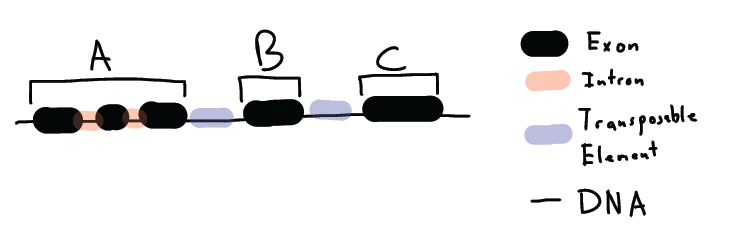
\includegraphics[width=100mm]{images/minute_gene_block.png}
\caption{A small haploid block of DNA from the ancestral chromosome of \emph{U. gibba}, showing features according to the legend.  The segment contains 3 genes named A, B, and C.}
\label{minute}
  \end{center}
\end{figure*}

\end{enumerate}
\end{document}
